\section{应用结果展示}  
%\label{chp:display}
在本节中,我们会对RunDroid运行结果做出相应的展示,并将展现结果和静态分析工具FlowDroid做对比,比较两个工具的产出结果,分析各自的优劣。

我们研究的APK的主体代码如\autoref{fig:code_demo}所示。
在\autoref{fig:code_demo}中,我们声明了有Activity\code{MainActivity},他是应用层的主Activity,该Activity界面主要有3个按钮组成,方便对应的是斐波拉契数量的计算、基于Handler的异步事件以及启动一个Activity(生命周期相关)。



\begin{figure}[!ht]
	\centering
	\begin{lstlisting}[language=Java]
package cn.mijack.rundroidtest;

public class MainActivity extends Activity implements View.OnClickListener {
	Button button1,button2,button3;
	Handler handler = new Handler() {
		public void handleMessage(Message msg) {
			if (msg.what == 1)    
			      Toast.makeText(MainActivity.this, "handle", Toast.LENGTH_SHORT).show();
		}
	};
	protected void onCreate(Bundle savedInstanceState) {
		super.onCreate(savedInstanceState);
		setContentView(R.layout.activity_main);
		button1 = findViewById(R.id.button1);
		button1.setOnClickListener(this);  // button2、button3进行相同的操作,此处省略
	}
	public void onClick(View view) {
		switch (view.getId()) {
			case R.id.button1:
				doHandleButton1();
				return;				// button2、button3进行相同的操作,此处省略
		}
	}
	public void doHandleButton1() {
		int fibonacci = doFibonacci(5);
		Toast.makeText(this, "fibonacci: " + fibonacci, Toast.LENGTH_SHORT).show();
	}
	private int doFibonacci(int i) {
		if (i <= 0)    return -1;   
		if (i == 1 || i == 2)   return 1; 
		return doFibonacci(i - 1) + doFibonacci(i - 2);
	}
	public void doHandleButton2() {
		Message message = Message.obtain();
		message.what = 1;
		handler.sendMessage(message);
	}
	public void doHandleButton3() {
		startActivity(new Intent(this, NewActivity.class));
	}
}\end{lstlisting}
%	\vspace{-9px}
	\caption{待测试APK的主体代码}
	\label{fig:code_demo}
\end{figure}

\subsection{函数调用图的构建结果展示}

在应用程序运行时,点击按钮button1,应用会计算斐波拉契数列中的第5项,并将这个数以Toast的形式展示给用户。
上述过程中,方法调用同时涉及到普通方法调用、递归函数调用。
RunDroid的动态分析结果如\autoref{fig:rundroid-result-Fibonacci}所示:
每一个红色节点对应的是一次方法执行,每一个绿色节点对应是一个对象;
如果对象是方法执行的方法对象,则在图中会有一条边从方法指向该对象,并在边上标识两种之间的关系(参数关系、返回值关系、实例关系等);
如果两个方法执行之间存在调用关系,则他们之间会通过从调用发起方指向被调用方的有向边进行连接。

在本案例中,\code{doHandleButton1()}调用了方法\code{doFibonacci()},因此前者有条有向边指向后者;
通过观察虚线框中各节点的关系,我们知道,对于方法\code{doFibonacci()},当参数为\question{5}时,对应的结果为\question{5}。

FlowDroid的静态分析结果如\autoref{fig:flowdroid-result-Fibonacci}所示。
通过比较\autoref{fig:rundroid-result-Fibonacci}和\autoref{fig:flowdroid-result-Fibonacci},我们可以发现以下有趣的结论:

首先,两者在方法\code{doFibonacci()}数量上不同的:RunDroid得到的结果中,方法节点\code{doFibonacci()}共有\question{9}个,即在运行过程中,\code{doFibonacci()}被调用了\question{9}次。
由于在一个应用中,一个方法的方法签名是唯一的,所以FlowDroid给出的结果中\code{doFibonacci()}只有一个。
另外,静态分析方法(FlowDroid)在分析\code{doFibonacci()}这类方法时,对函数的执行上下文做出准确的判断,进而给出程序准确的运行时行为。
因此,静态分析技术得到的函数调用图往往以方法体本身作为研究的基本单元,而动态分析技术的函数调用图可以细化方法执行之间的关系,在一定程度上可以反映程序执行的具体过程。


\begin{figure*}[!ht]
	\centering
	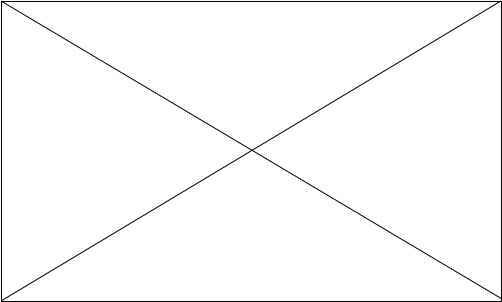
\includegraphics[width=\textwidth]{./Figures/empty.png}
	\caption{斐波拉契数列-RunDroid生成的调用图}
	\label{fig:rundroid-result-Fibonacci}
\end{figure*}

其次,方法\code{Toast.makeText(Context,CharSequence,int)}没有出现在RunDroid的结果中,而FlowDroid给出的结果却有展现:
而在运行过程中,我们却可以看到Toast提示。
经过分析,原因如下:\code{Toast.makeText(Context,CharSequence,int)}属于系统定义的方法,而运行时拦截器待拦截的方法列表中并未包含该方法,因此运行时未收集到相关的方法执行信息,导致RunDroid无法在调用图中还原相应的函数。
这也从一个方面反映了RunDroid的劣势:系统函数运行时信息的捕获需要提前将相应的方法告知运行时拦截器,生成的调用图才会包括相应的方法。
这使得调用图只包含研究人员关心的方法的执行信息,但也在一定程度上导致部分方法的缺失和调用图的局部不完整。


\begin{figure*}[!ht]
	\centering
	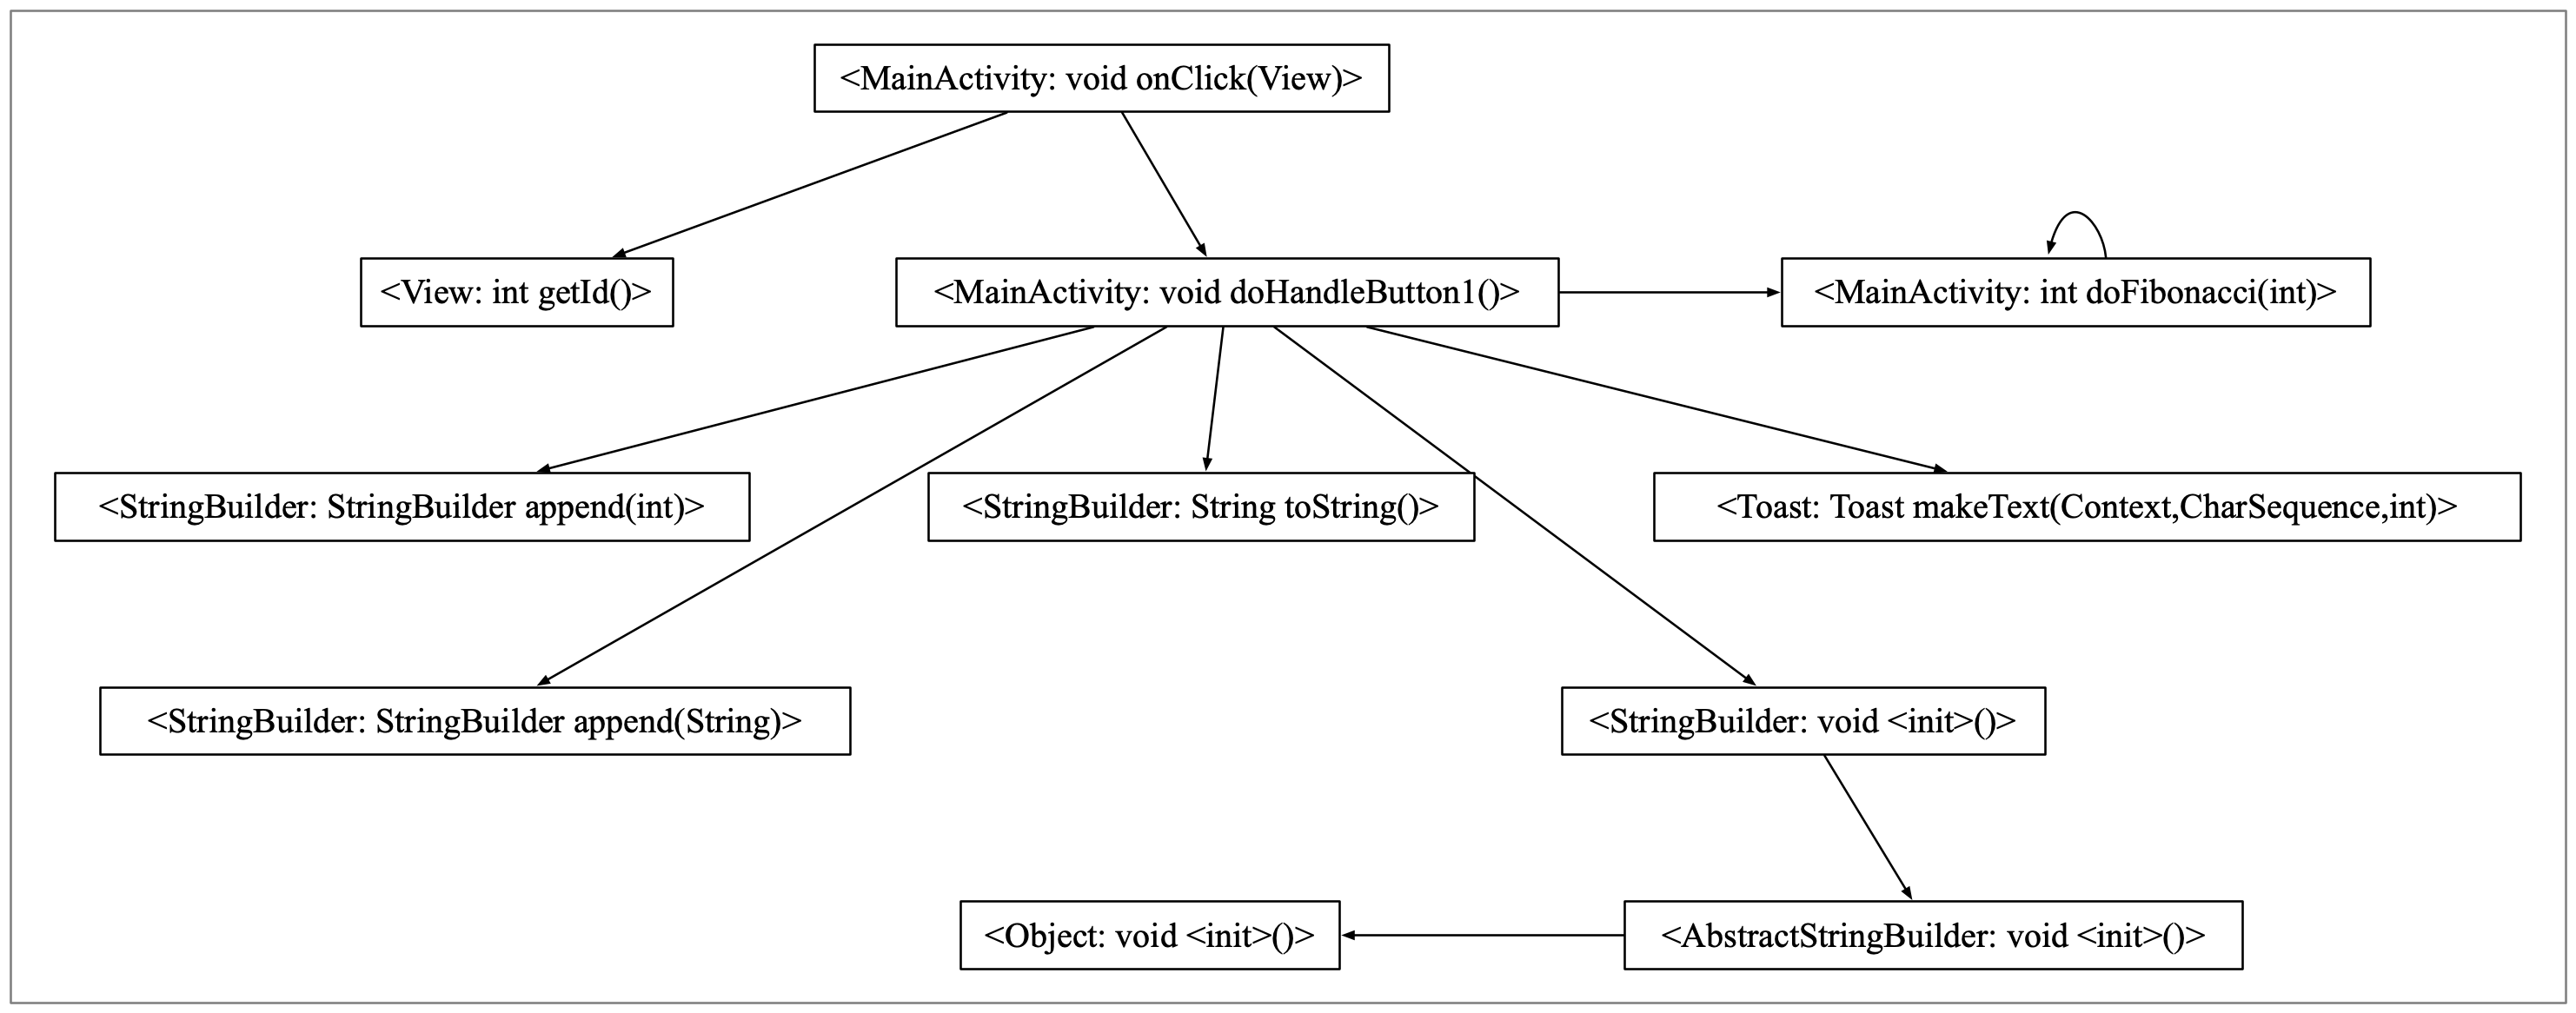
\includegraphics[width=\textwidth]{./Figures/FlowDroid-Fibonacci.png}
	\caption{斐波拉契数列-FlowDroid生成的调用图}
	\label{fig:flowdroid-result-Fibonacci}
\end{figure*}


最后,FlowDroid给出的结果中包括了大量和\code{StringBuilder}相关的方法,而RunDroid的结果并不包括这些方法:
对比源码发现,源程序并未直接使用\code{StringBuilder}。
通过查阅文献\cite{gosling2000java},我们发现出于提高字符串串联性能的考虑,Java编译器可以使用类\code{StringBuilder}等技术通过源代码做适当等价的修改,以避免表达式求值过程中产生过多的字符串数量。
由于上述过程发生在Java程序编译阶段并最后以字节码的形式不存在APK文件中,而FlowDroid恰好从字节码层面对应用进行分析,因此FlowDroid的分析结果会包含该方法。
对于RunDroid,上述方法既在源代码中未出现相关方法定义(无法进行日志代码编织),又不在运行时拦截器的目标方法列表中,所以RunDroid给出的调用图自然也不会包括\code{StringBuilder}相关的方法。



\subsection{Activity的生命周期效果展示}

这本小节中,应用运行时,我们将点击按钮button2,在\code{MainActivity}启动另一个\code{NewActivity},对比RunDroid和FlowDroid在Activity生命周期方法的呈现效果。
RunDroid的运行结果如\autoref{fig:rundroid-result-lifecycle}所示,FlowDroid的静态分析结果如\autoref{fig:flowdroid-result-lifecycle}所示。

\begin{figure*}[ht]
	\centering
	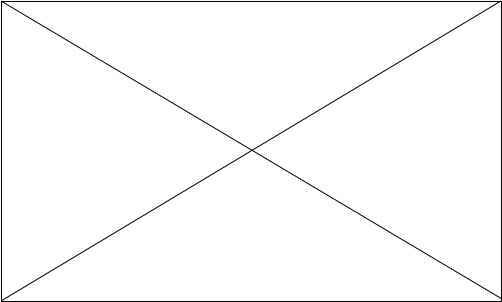
\includegraphics[width=\textwidth]{./Figures/empty.png}
	\caption{RunDroid生成的调用图-Activity部分}
	\label{fig:rundroid-result-lifecycle}
\end{figure*}


\begin{figure*}[ht]
	\centering
	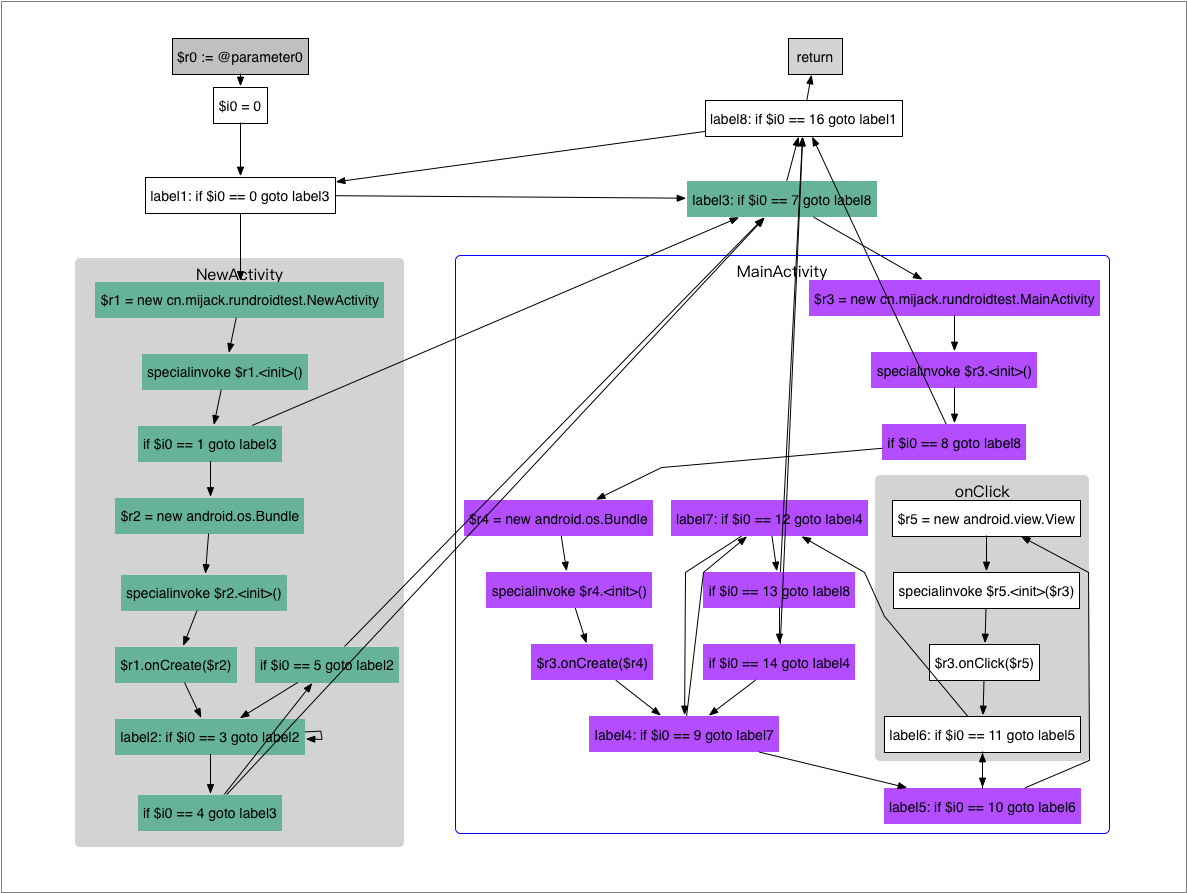
\includegraphics[width=\textwidth]{./Figures/flowdroid-dummyMainMethod.png}
	\caption{dummyMainMethod-FlowDroid生成的调用图}
	\label{fig:flowdroid-result-lifecycle}
\end{figure*}


\subsection{多线程触发关系效果展示}

\begin{figure*}[ht]
	\centering
	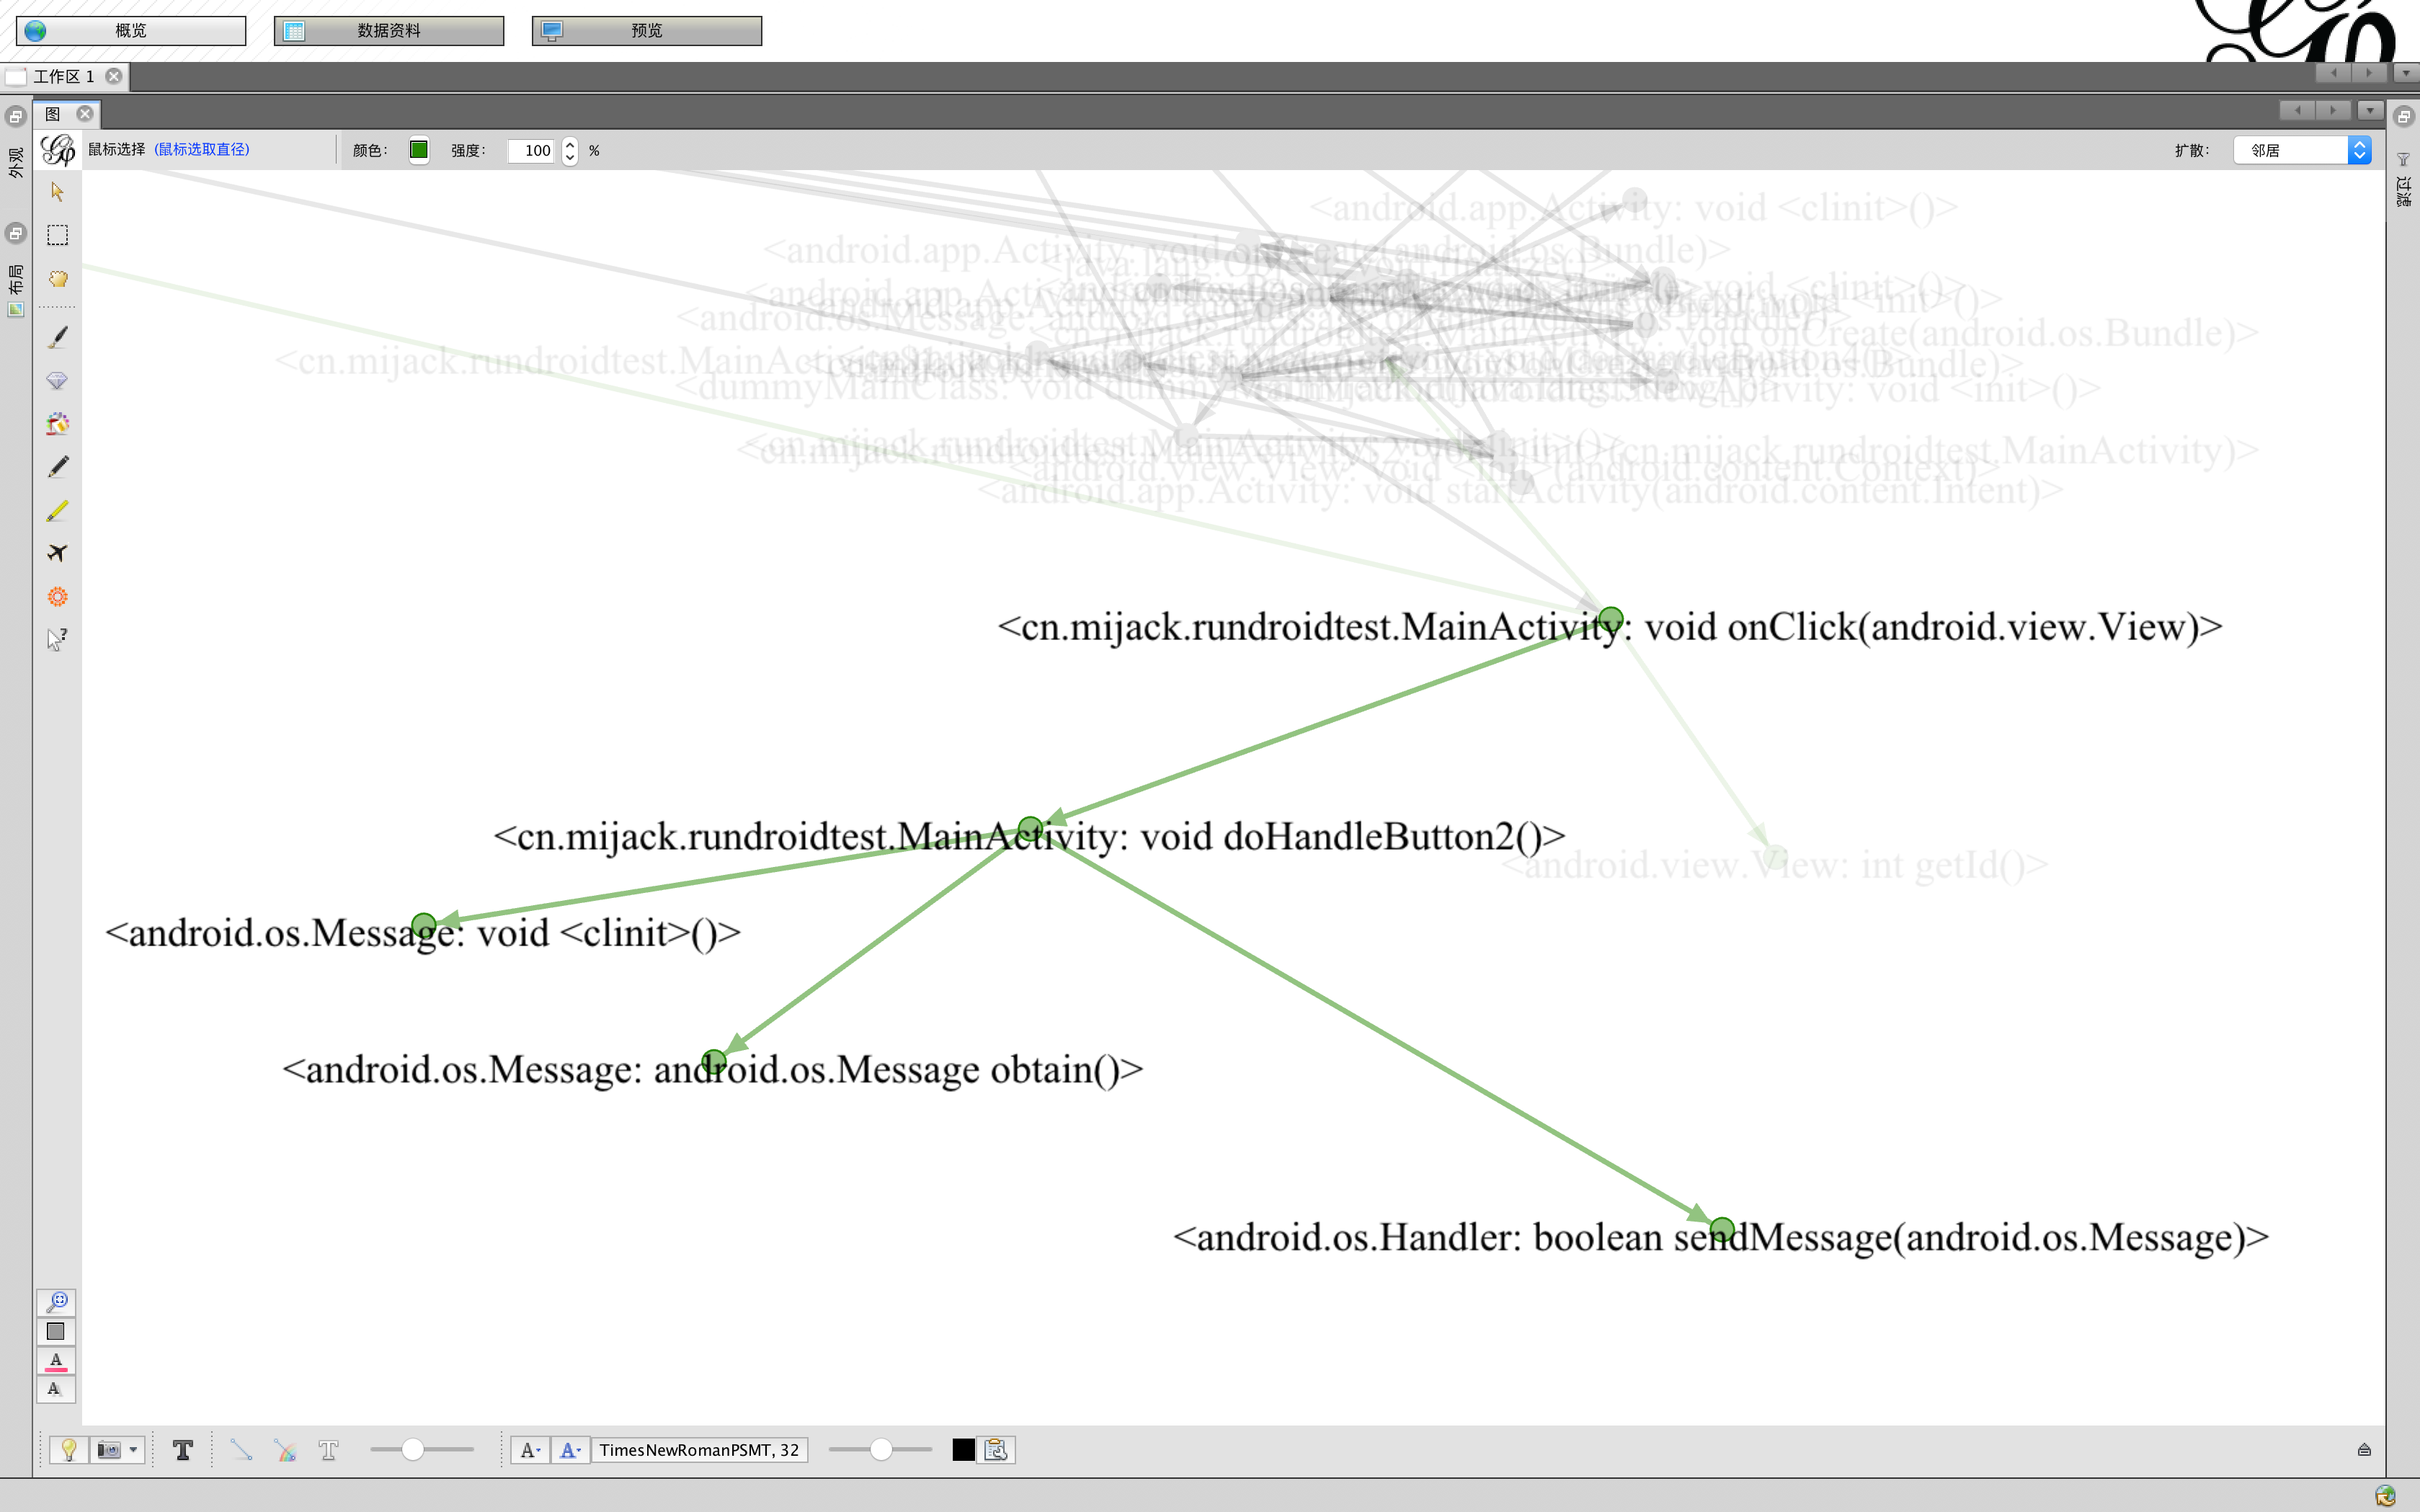
\includegraphics[width=\textwidth]{./Figures/FlowDroid-handler.png}
	\caption{Handler-FlowDroid生成的调用图}
	\label{fig:flowdroid-result-handler}
\end{figure*}
 \section{本章小结}
 
% 本章中,我们将环绕着构建效率、日志效率、运行效率等三个方面对RunDroid角进行系统性能测试和评估,并结合实验结果阐述了采用源代码插桩、基于MMap的日志方案等原因。
 
本章中展示RunDroid系统生成的函数调用图的运行结果,并对函数调用图进行详细的阐述。
